% !TeX program = xelatex
% !TeX encoding = utf8
% !TeX root = Elo1_HS22.tex

%% TODO: publish to CTAN
\documentclass[margin=normal]{tex/hsrzf}

%%%%%%%%%%%%%%%%%%%%%%%%%%%%%%%%%%%%%%%%%%%%%%%%%%%
% Packages

%% TODO: publish to CTAN
\usepackage{tex/hsrstud}

%% Language configuration
\usepackage{polyglossia}
\usepackage{multicol}
\usepackage{tikz}
\usepackage[european]{circuitikz}
\setdefaultlanguage[variant=swiss]{german}

%% License configuration
\usepackage[
    type={CC},
    modifier={by-nc-sa},
    version={4.0},
    lang={german},
]{doclicense}

%%%%%%%%%%%%%%%%%%%%%%%%%%%%%%%%%%%%%%%%%%%%%%%%%%%
% Metadata

\course{Elektrotechnik}
\module{ModAbk}
\semester{Herbstsemester 2022}

\authoremail{joel.leirer@ost.ch}
\author{\textsl{Joël Leirer} -- \texttt{\theauthoremail}}

% did someone help you with this work?
\contributors{

  % do not forget to add yourself!
}

\title{\texttt{\themodule} Zusammenfassung}
\date{\thesemester}

%%%%%%%%%%%%%%%%%%%%%%%%%%%%%%%%%%%%%%%%%%%%%%%%%%%
% Document

\begin{document}

% use roman numberals for introductiory pages
\pagenumbering{roman}

\maketitle

% \begin{abstract}
% \end{abstract}

% show the names of the people who contributed to this document.
% \section*{Contributors}
% \thecontributors

\section*{Lizenz}
\doclicenseThis

\clearpage
\tableofcontents

% actual content
\clearpage
\setcounter{page}{1}
\pagenumbering{arabic}

\section{Arbeitspunktbestimmung}
AC und DC Teile der Schaltung separat anschauen.
\subsection{DC}
\begin{itemize}
  \item Grosssignalwiderstung ($\frac{U}{I}$) 
  \item AC-Quellen "Abschalten", AC-Quellen mit DC Anteil durch DC-Quellen ersetzen
  \item Kondensatoren entfernen (Unterbruch)
  \item Spule Kurschliessen
\end{itemize}
\subsection{AC}
\begin{itemize}
  \item Kleinsignalwiderstand (Impedanz,$\frac{dU}{dI}$ )
  \item DC-Quellen "Abschalten" (U --> Kurzschluss, I --> Unterbruch)
  \item Nichtlineare Bauteil durch ihre Kleinsignal Ersatzschaltung ersetzen
  \item Koppel- und Bypass-Kondensatoren kurzschliessen
  \item Sperrdrosseln ("grossse" Induktivitäten) entfernen (Unterbruch)
\end{itemize}

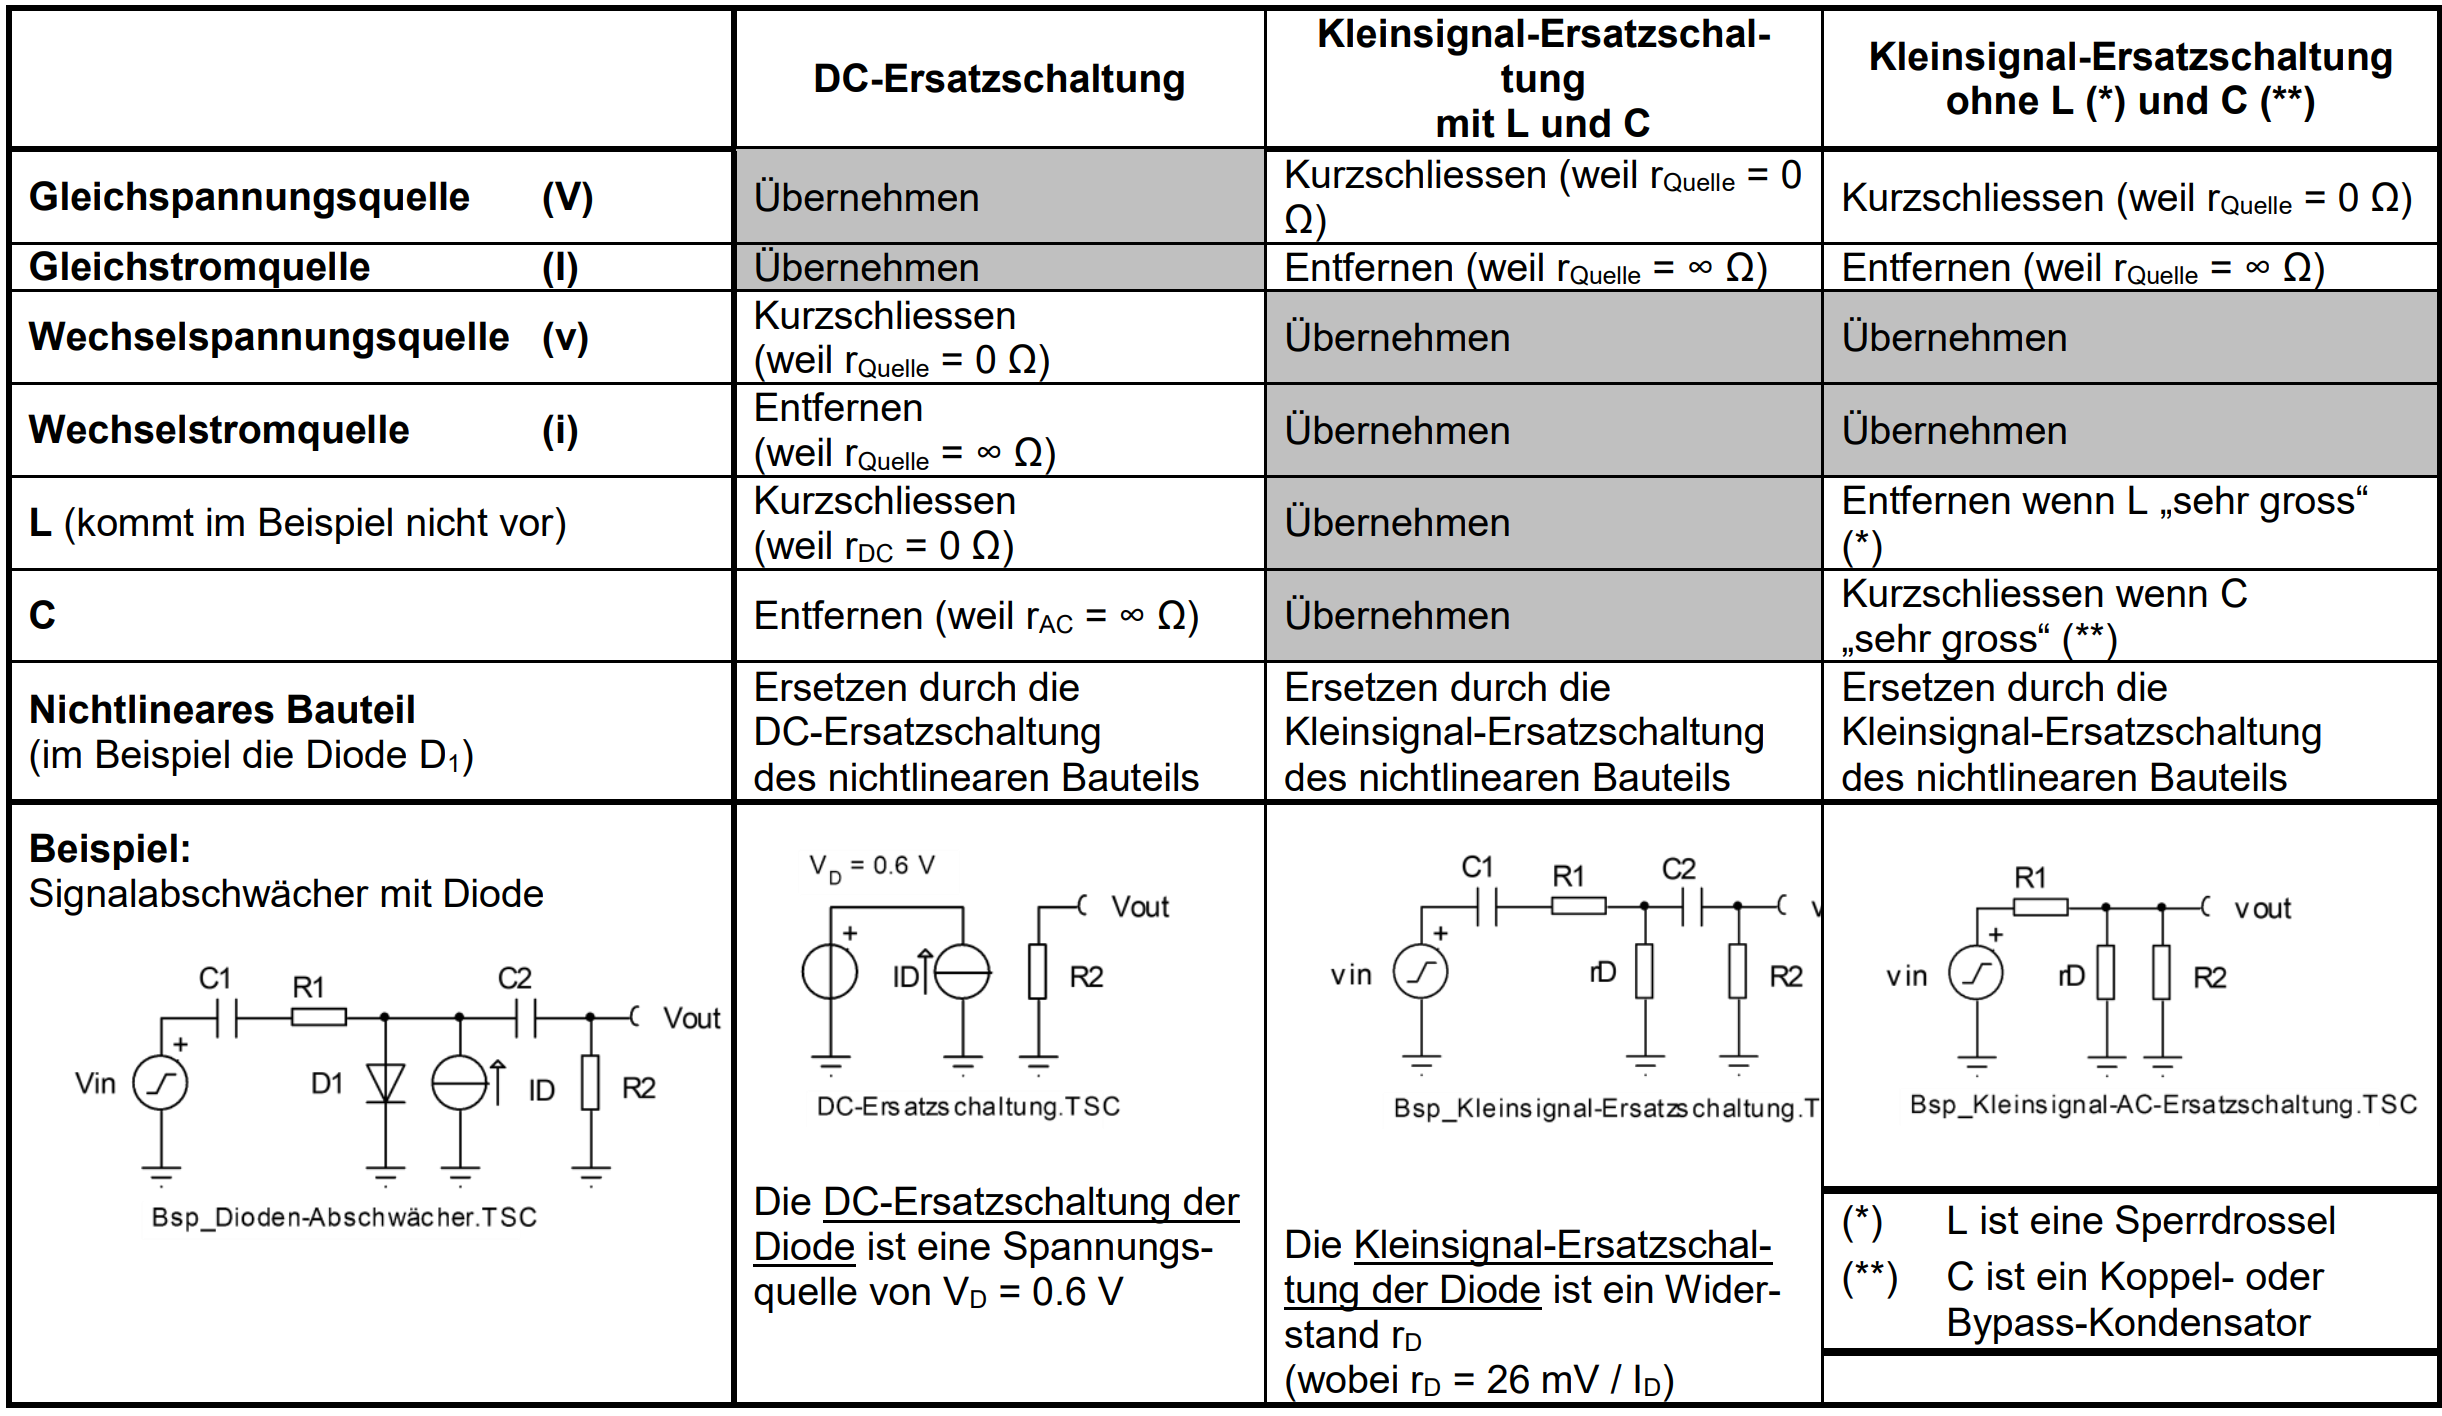
\includegraphics[width = 5cm]{img/Tabelle Kleinsignal Ersatzschaltung.png}

\section{OpAmp}
\subsection{negative Rückkopplung}
\subsubsection*{Nicht Invertierender Verstärker}
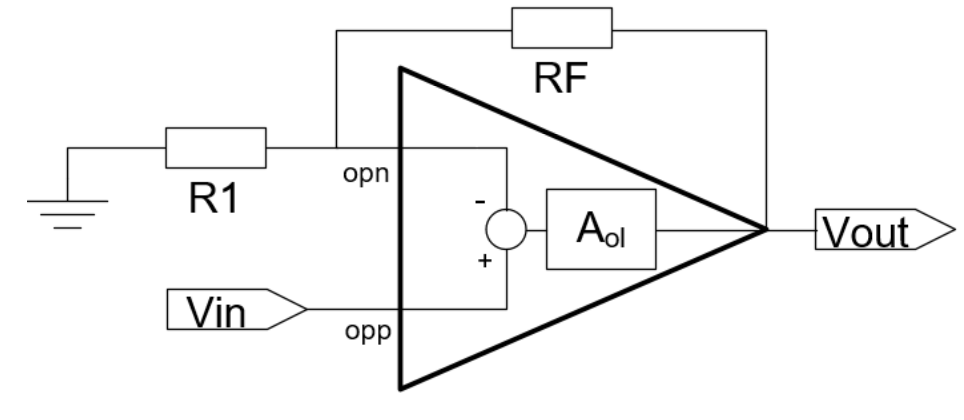
\includegraphics[width = 5cm]{img/OpAmp/Verstaerker_nicht_invertierend.png}
\subsubsection*{Invertierender Verstärker}
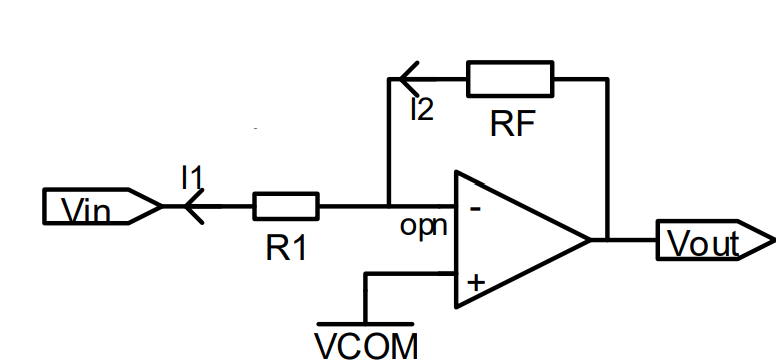
\includegraphics{img/OpAmp/Verstaerker_invertierend.png}
\subsubsection*{Summierender Verstärker}
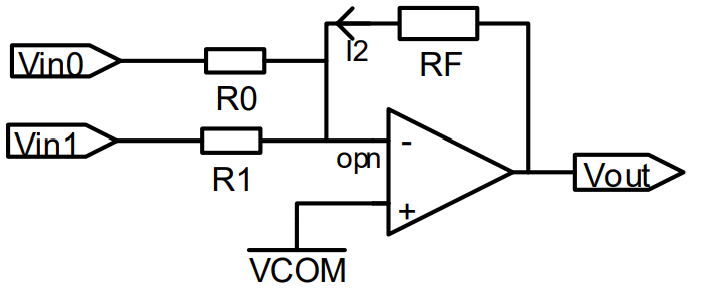
\includegraphics{img/OpAmp/Verstaerker_summierend.png}
\subsubsection*{Buffer}
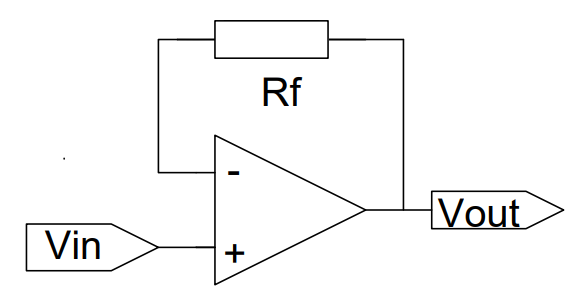
\includegraphics{img/OpAmp/Buffer.png}


\end{document}
